\documentclass{article}
\usepackage[utf8]{inputenc}

\title{Homework 3 Report}
\author{Benny Chen}
\date{\today}
 
\usepackage{color}
\usepackage{amsthm}
\usepackage{amssymb} 
\usepackage{amsmath}
\usepackage{listings}
\usepackage{xcolor}
\usepackage{listings}
\usepackage{graphicx}
\usepackage[hidelinks]{hyperref}
\usepackage{courier} 

\lstset{
tabsize = 4, %% set tab space width
showstringspaces = false, %% prevent space marking in strings, string is defined as the text that is generally printed directly to the console
numbers = left, %% display line numbers on the left
commentstyle = \color{green}, %% set comment color
keywordstyle = \color{blue}, %% set keyword color
stringstyle = \color{red}, %% set string color
rulecolor = \color{black}, %% set frame color to avoid being affected by text color
basicstyle = \small \ttfamily , %% set listing font and size
breaklines = true, %% enable line breaking
numberstyle = \tiny,
}

\begin{document}
\maketitle

\section*{Problem A}
Upgrade the program VendingChange.java from Homework \#1 to prompt the user to enter the input price. The program then checks whether the input price entered by the user conforms to the specifications. Recall that the two constraints on the input price are: (i) it should be more than 25c but less than 100c; both inclusive and (ii) it should be a multiple of 5. If either of these conditions is not met, the program should print a message “Invalid Input” and prompt the user to enter a new input. This process must be repeated until the user provides a valid price.

\begin{center}
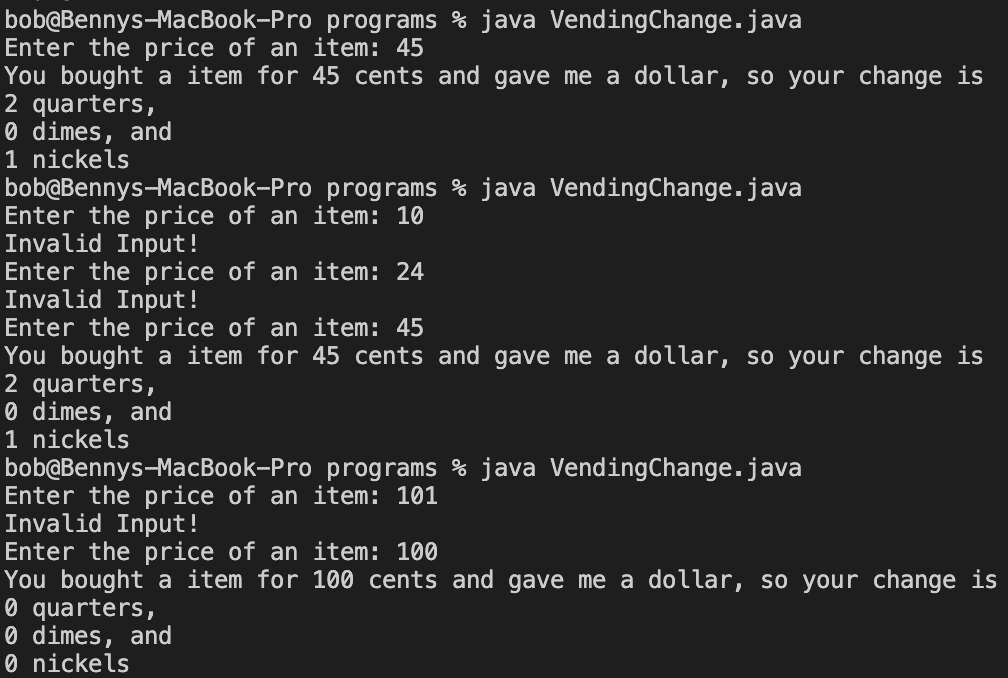
\includegraphics[width=\textwidth]{./images/vending.png}
\end{center}

\section*{Problem B}
Write a program BMIClassification.java that prompts the user to input their weight (in pounds) and height (in inches). Note that both the weight and height can be real. The program then converts the weight to kilograms and height to meters, and calculates the BMI according to the equation:

\[BMI = weight/(height^2)\]

\noindent
The program prints the BMI of the user. Further, based on the value of the BMI, the program produces the risk classification of the user according to the following rules.
\begin{itemize}
    \item Underweight – less than 18.5
    \item Normal weight – greater than or equal to 18.5 and less than 25
    \item Overweight – greater than or equal to 25 and less than 30
    \item Obese – greater than or equal to 30.
\end{itemize}

\begin{center}
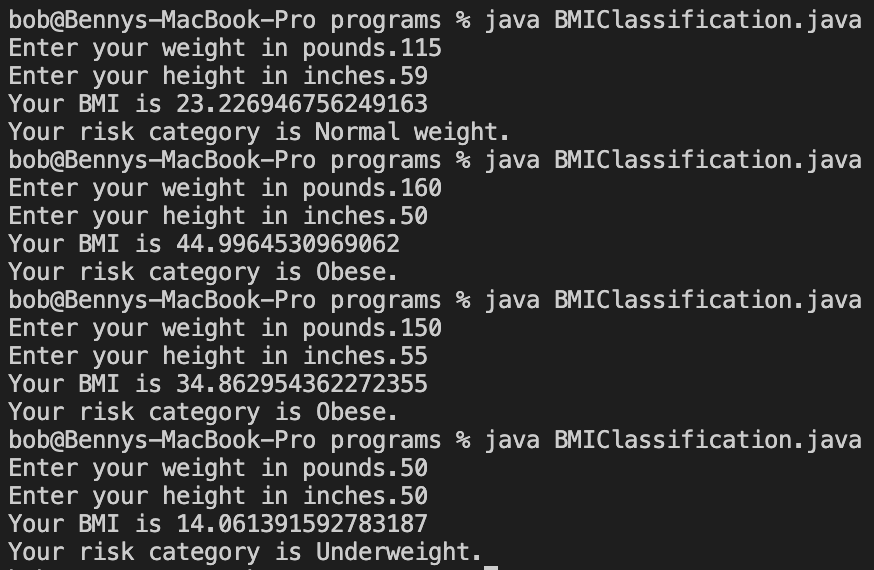
\includegraphics[width=\textwidth]{./images/BMIclass.png}
\end{center}

\section*{Problem C}
Write a program TaylorSeries.java that calculates ex as a sum of the first n terms of the following Taylor series:

\[e^x = 1 + x +\ldots+\frac{x^n}{n!}\]

\noindent
The program should prompt the user to input n and x, and print ex as output, accurate up to two decimal places. n is an integer and x is a real number.

\begin{center}
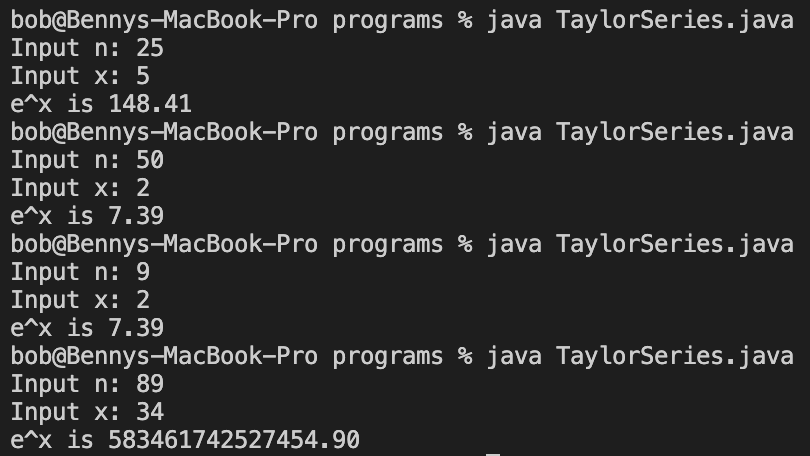
\includegraphics[width=\textwidth]{./images/taylor.png}
\end{center}

\section*{Problem D}

The transactions at a store are saved in a txt file with the following pre-specified format:

\noindent
SKU,Quantity,Price,Description 
\begin{itemize}
    \item 4039,50,0.99,SODA
    \item 9100,5,9.50,T-SHIRT
    \item 1949,30,110.00,JAVA PROGRAMMING TEXTBOOK
    \item 5199,25,1.50,COOKIE
\end{itemize}
Write a program TransactionReport.java that prompts the user for the name of the input file, reads the transactions from the file, after skipping over the first line which is the header. The program then produces a transaction report by first computing the sale amount for each item as a product of the quantity and price, and then computing the total sale across all the items. Thus, the output produced by processing the above file is as follows.

\subsection*{Test Cases}
Trans.txt:

\begin{itemize}
    \item SKU,Quantity,Price,Description 
    \item 4039,50,0.99,SODA
    \item 9100,5,9.50,T-SHIRT
    \item 1949,30,110.00,JAVA PROGRAMMING TEXTBOOK 
    \item 5199,25,1.50,COOKIE
\end{itemize}

\noindent
Trans2.txt:

\begin{itemize}
    \item SKU,Quantity,Price,Description 
    \item 4039,1,0.99,SODA
    \item 9100,1,9.99,T-SHIRT
\end{itemize}

\noindent
Trans3.txt:

\begin{itemize}
    \item SKU,Quantity,Price,Description 
    \item 4039,0,0.99,SODA
    \item 9100,50,9.50,T-SHIRT
    \item 9101,50,9.50,T-SHIRT
    \item 1949,30,110.00,JAVA PROGRAMMING TEXTBOOK 
    \item 5199,5,.50,CHIPS
    \item 1949,3,110.00,JAVA PROGRAMMING TEXTBOOK 
    \item 5199,1,1.50,COOKIE
\end{itemize}
\begin{center}
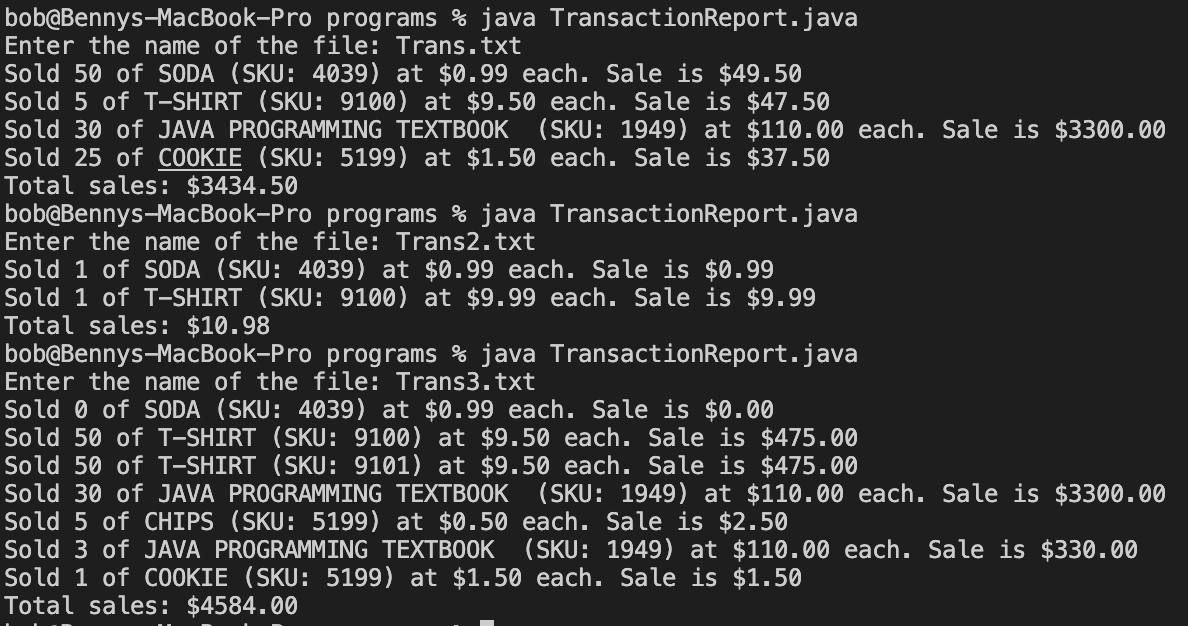
\includegraphics[width=\textwidth]{./images/Transaction.png}
\end{center}

\end{document}